\subsubsection{Beispiel für zweidimensionales Array}
Wir werden mit einem Array vom Typ \Tchar arbeiten, was bedeutet, dass jedes Element nur ein Byte Speicherplatz
benötigt.


\myparagraph{Beispiel: Zeile füllen}
\myindex{\olly}
Füllen wir die zweite Zeilen mit den Werten 0..3:

\lstinputlisting[caption=Row filling example,style=customc]{patterns/13_arrays/5_multidimensional/two1_DE.c}
Alle drei Zeilen sind rot markiert.
Wir erkennen, dass die zweite Zeilen nun die Werte 0,1,2 und 3 enthält:

\begin{figure}[H]
\centering
\includegraphics[width=0.6\textwidth]{patterns/13_arrays/5_multidimensional/olly_2D_1.png}
\caption{\olly: Array ist befüllt}
\end{figure}

\myparagraph{Beipsiel: Spalte füllen}
\myindex{\olly}
Füllen wir die dritte Spalte mit den Werten 0..2:

\lstinputlisting[caption=Column filling example,style=customc]{patterns/13_arrays/5_multidimensional/two2_DE.c}

Die drei Spalten sind hier ebenfalls rot markiert.

Wir erkennen, dass sich in jeder Zeile an der dritten Stelle die Werte 0,1 und 2 befinden. 

\begin{figure}[H]
\centering
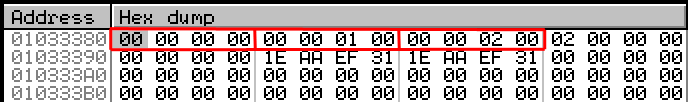
\includegraphics[width=0.6\textwidth]{patterns/13_arrays/5_multidimensional/olly_2D_2.png}
\caption{\olly: Array ist befüllt}
\end{figure}

